\documentclass[14pt]{beamer}
\title[CP01.13 BC]{JEE :: Introduction to JDBC}
\author[TS]{TalentSprint}
\institute[L\&D]{Licensed To Skill}
\date{Version 1.0.4}
\usefonttheme{serif}
\usecolortheme{orchid}
\usepackage{bookman}
\usepackage{hyperref}
\usepackage[T1]{fontenc}
\usepackage{graphicx}
\usepackage{listings}
\usepackage{multicol}
\graphicspath{{../../Images/}}
%\graphicspath{{Images/}}
\lstset{language=Java,numbers=left, numberstyle=\tiny, basicstyle=\footnotesize, numbersep=10pt, showstringspaces=false, breaklines=true,keepspaces=true, columns=flexible}
\beamertemplateballitem
\usebackgroundtemplate{
\includegraphics[width=\paperwidth]{TS-Logo.jpg}}

\begin{document}
\begin{frame}
  \titlepage
\end{frame}

\begin{frame}{Introduction to JDBC}
The content in this presentation is aimed at teaching  learners to:
\begin{itemize}
  \item Identify the types of Drivers
  \item List the Pros and Cons of JDBC Drivers
  \item Establish connection using Type-4 Driver
  \item Retrive/Insert/Update the data in/form Database
\end{itemize}
\end{frame}


\begin{frame}{Introduction to JDBC}
The content in this presentation is aimed at teaching  learners to:
\begin{itemize}
  \item Use different type of Statements
  \item Use different type of ResultSet
  \item Perform Batch Operations
  \item Get the Meta data of the Database and ResultSet
\end{itemize}
\end{frame}

\begin{frame}{Introduction to JDBC}
The content in this presentation is aimed at teaching  learners to:
\begin{itemize}
  \item Understanding PreparedStatement
  \item Flow of PreparedStatement working
  \item Programming Interaction
\end{itemize}
\end{frame}


\begin{frame}{Introduction to JDBC}
\begin{block}{}
JDBC (Java DataBase Connectivity)
\end{block}

\begin{itemize}
\item A sub set of CLI (Call Level Interface) specification.
\item Can Create a platform-neutral interface between Java applications and Databases.
\item Contains standard functions required to connect and perform SQL operation on the DB
\item Communicates with ODBC , DB native libraries , java socket connection to DB
\end{itemize}
\end{frame}

\begin{frame}{Introduction to JDBC}
\begin{block}{}
Why JDBC?
\end{block}

\begin{itemize}
\item To enable a java application to interact with a database
\item To provides a common base on which alternate interfaces and tools can be built
\end{itemize}
\end{frame}

\begin{frame}{Introduction to JDBC}
\begin{block}{}
Why JDBC?
\end{block}

\begin{center}
    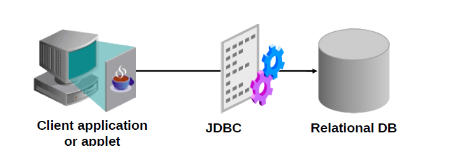
\includegraphics[scale=0.5]{JEE-M03-S01-Image1.png}
  \end{center}
\end{frame}

\begin{frame}{Introduction to JDBC}
\begin{block}{}
Driver Types
\end{block}
There are four types of  JDBC drivers available in java for connecting to Database
\begin{description}
\item [Type 1] JDBC-ODBC Bridge plus ODBC Driver
\item [Type 2] Native API Partly Java Driver
\item [Type 3] JDBC -Net pure Java Driver
\item [Type 4] Native-Protocol Pure Java Driver
\end{description}
\end{frame}

\begin{frame}{Introduction to JDBC}
\begin{block}{}
  Type 1 - JDBC-ODBC Bridge plus ODBC Driver
\end{block}
\begin{itemize}
\item Translates the JDBC method calls into ODBC function calls.
\item Included with the JDK in the sun.jdbc.odbc.JdbcOdbcDriver class.
\item Not recommended for production use.
\end{itemize}
\end{frame}

\begin{frame}{Introduction to JDBC}
\begin{center}
    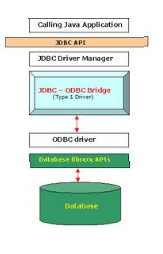
\includegraphics[scale=0.5]{JEE-M03-S01-Image2.png}
  \end{center}
\end{frame}



\begin{frame}{Introduction to JDBC}
\begin{block}{}
  Type 2 - Native API Partly Java Driver
\end{block}
\begin{itemize}
\item Partly written in Java and partly in the native code. So, called Native API Partly Java Driver.
\item Consists of drivers that communicate with databases servers in the server’s native protocol.
\item Implemented in a combination of binary code and Java.
\end{itemize}
\end{frame}

\begin{frame}{Introduction to JDBC}
\begin{itemize}
\item Installation is easier than installing both the JDBC-ODBC bridge and an ODBC driver.
\end{itemize}
\begin{center}
    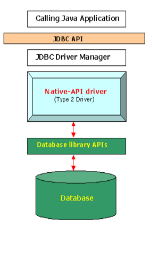
\includegraphics[scale=0.5]{JEE-M03-S01-Image3.png}
  \end{center}
\end{frame}

\begin{frame}{Introduction to JDBC}
\begin{block}{}
  Type 3 -  JDBC -Net pure Java Driver
\end{block}
\begin{itemize}
\item Communicate with a database access server using HTTP or SHTTP protocol and works for both the Internet and the Intranet.
\item Translates the network protocol into a vendor specific database protocol
\item Served from the web server are the best solution for the applets.
\end{itemize}
\end{frame}

\begin{frame}{Introduction to JDBC}
\begin{itemize}
\item Automatically installed on the user’s machine in a transparent manner.
\end{itemize}
\begin{center}
    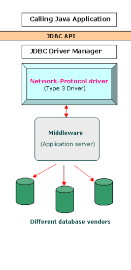
\includegraphics[scale=0.5]{JEE-M03-S01-Image4.png}
  \end{center}
\end{frame}

\begin{frame}{Introduction to JDBC}
\begin{block}{}
  Type 4 -  Native-Protocol Pure Java Driver
\end{block}
\begin{itemize}
\item A pure Java library that translates JDBC calls directly to a database-specific protocol.
\item Written completely in Java and is hence platform independent.
\item Installed inside the Java Virtual Machine of the client.
\end{itemize}
\end{frame}

\begin{frame}{Introduction to JDBC}
\begin{itemize}
\item Does not have the overhead of conversion of calls into ODBC or database API calls.
\item Efficient for Intranet applications.
\end{itemize}
\begin{center}
    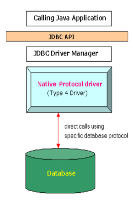
\includegraphics[scale=0.5]{JEE-M03-S01-Image5.png}
  \end{center}
\end{frame}


\begin{frame}{Introduction to JDBC}
\begin{block}{}
JDBC Specifications
\end{block}
Consists of the following interfaces and classes:
\begin{center}
    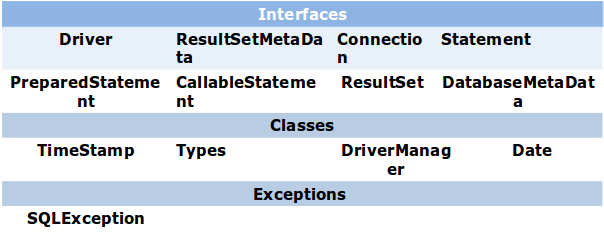
\includegraphics[scale=0.5]{JEE-M03-S01-Image6.png}
  \end{center}
\end{frame}


\begin{frame}{Introduction to JDBC}
\begin{block}{}
Steps to establish a connection 
\end{block}
\begin{center}
    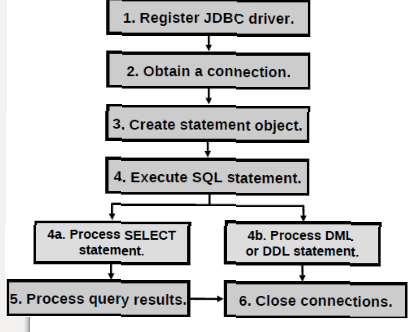
\includegraphics[scale=0.5]{JEE-M03-S01-Image7.png}
  \end{center}
\end{frame}

\begin{frame}[fragile]{Introduction to JDBC}
\begin{block}{}
Steps to establish a connection 
\end{block}
\begin{block}{}
Step 1 - Load/Register JDBC Drivers
\end{block}
Before the driver manager can activate a driver, the driver must be registered manually by loading its class using the ``Class'' class
\textbf{Example}
\begin{itemize}
\item JDBC-ODBC Bridge driver
\begin{lstlisting}[numbers=none]
Class.forName(``sun.jdbc.odbc.JdbcOdbcDriver'');
\end{lstlisting}
\end{itemize}
\end{frame}
\begin{frame}[fragile]{Introduction to JDBC}
\begin{itemize}
\item Native-Protocol Pure Java Driver 
\begin{lstlisting}[numbers=none]
Class.forName(``sun.jdbc.odbc.JdbcOdbcDriver'');
\end{lstlisting}
\item Oracle 
\begin{lstlisting}[numbers=none]
Class.forName(``oracle.jdbc.driver.OracleDriver'');
\end{lstlisting}
\item MySql
\begin{lstlisting}[numbers=none]
 Class.forName(``com.mysql.jdbc.Driver'');
\end{lstlisting}
\end{itemize}
\end{frame}


\begin{frame}{Introduction to JDBC}
\begin{block}{}
Steps to establish a connection 
\end{block}
\begin{block}{}
Step 2 -  Establish Connection using Driver Manager
\end{block}

\begin{itemize}
\item Select the database drivers 
\item Create a new database connection by calling the static method getConnection() of the DriverManager class
\end{itemize}
\end{frame}

\begin{frame}{Introduction to JDBC}
\begin{itemize}
\item This method takes
\begin{itemize} 
\item the database URL 
\item a user name    // Optional 
\item password       // Optional
\end{itemize}
\end{itemize}
\end{frame}


\begin{frame}{Introduction to JDBC}
\begin{block}{}
JDBC URLs
\end{block}
\begin{itemize} 
\item JDBC uses a URl-like string. The URL identifies.
\item Database connection details, vary depending on the driver used.
\end{itemize}
\begin{center}
    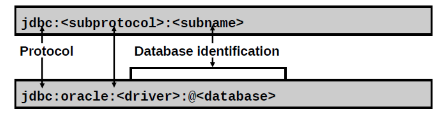
\includegraphics[scale=0.5]{JEE-M03-S01-Image8.png}
  \end{center}
\end{frame}
\begin{frame}{Introduction to JDBC}
\begin{itemize} 
\item jdbc:oracle:thin:@localhost:1521:orcl --For Oracle SE
\item jdbc:oracle:thin:@localhost:1521:XE --For Oracle XE
\item jdbc:mysql://localhost:3306/dbname --For MySql
\end{itemize}
\end{frame}

\begin{frame}[fragile]{Introduction to JDBC}
\begin{block}{}
Steps to establish a connection 
\end{block}
\begin{block}{}
Step 3 - Create the Statement
\end{block}
Create one of the following Statement object to send SQL statement to the database using Connection Object (con).
\begin{description}
\item [Statement] executes a static SQL statement
\begin{lstlisting}[numbers=none]
Statement stmt= con.createStatement();
\end{lstlisting}
\end{description}
\end{frame}

\begin{frame}[fragile]{Introduction to JDBC}
\begin{description}
\item [PreparedStatement] represents a precompiled SQL statement
\begin{lstlisting}[numbers=none]
PreparedStatement ps=con.prepareStatement(query);
\end{lstlisting}
\item [CallableStatement] executes SQL stored procedures
\begin{lstlisting}[numbers=none]
CallableStatement cs=con.prepareCall(query);
\end{lstlisting}
\end{description}
\end{frame}


\begin{frame}{Introduction to JDBC}
\begin{block}{}
Steps to establish a connection 
\end{block}
\begin{block}{}
Step 4 - Execute the Statement
\end{block}

The Statement interface provides three methods to execute SQL statements:
\begin{itemize} 
\item Use executeQuery(String sql)for SELECT statements
\begin{itemize} 
\item Returns a ResultSet object for processing rows
\end{itemize}
\item Use executeUpdate(String sql) for DML or DDL
\begin{itemize} 
\item Returns an int  represents the row count for SQL Data Manipulation Language
\end{itemize}
\end{itemize}
\end{frame}

\begin{frame}{Introduction to JDBC}
\begin{itemize} 
\item Use execute(String) for any SQL statement.
\begin{itemize} 
\item Returns a boolean value, such that 
\begin{itemize}
\item if the first result is a ResultSet object returns true
\item if it is an update count or there are no results returns false
\end{itemize}
\end{itemize}
\end{itemize}
\end{frame}


\begin{frame}{Introduction to JDBC}
\begin{block}{}
Steps to establish a connection 
\end{block}
\begin{block}{}
Step 4a - Process SELECT Statement
\end{block}
Statement will returns the results of a query in a ResultSet object.
\begin{itemize} 
\item Maintains a cursor pointing to its current row of data
\item Provides following methods to retrieve column values
\begin{itemize} 
\item Use the next() method in loop to iterate through rows

\end{itemize}
\end{itemize}
\end{frame}

\begin{frame}[fragile]{Introduction to JDBC}
\begin{itemize} 
\item Use getXXX() methods to obtain column values by column  position in query, or column name.
\end{itemize}
\begin{lstlisting}[numbers=none]
ResultSet rs=stmt.executeQuery(``SELECT''+ ``ename, empno FROM emp'');
while(rs.next())
{
String s= rs.getString(``ename'');
int n = rs.getInt(``empno'');
System.out.println(s+ ``-'' + n);
}
\end{lstlisting}
\end{frame}

\begin{frame}[fragile]{Introduction to JDBC}
\begin{block}{}
Steps to establish a connection 
\end{block}
\begin{block}{}
Step 4b - Submitting DDL / DML Statement
\end{block}
\begin{description}
\item [DDL Statement] Create a table in a database from a JDBC program using the following lines of code:
\begin{lstlisting}[numbers=none]
String creatTable = ``CREATE TABLE emp''+``(ename VARCHAR2(32),empno NUMBER)'';
stmt.executeUpdate(createTable);
\end{lstlisting}
\end{description}
\end{frame}

\begin{frame}[fragile]{Introduction to JDBC}
\begin{description}
\item [DML Statement] Insert values into a table in from a JDBC program using the following lines of code:
\begin{lstlisting}[numbers=none]
stmt.executeUpdate(``INSERT INTO emp''+ ``VALUES(`Ram', `101')'');
\end{lstlisting}
\end{description}
\end{frame}


\begin{frame}[fragile]{Introduction to JDBC}
\begin{block}{}
Steps to establish a connection 
\end{block}
\begin{block}{}
Step 5 - Closing Connection
\end{block}
\begin{itemize}
\item Explicitly close a Connection, Statement, and ResultSet object to release resources that are no longer needed.
\item Protect the database from accidental changes.
\begin{lstlisting}[numbers=none]
rs.close();
stmt.close();
con.close();
\end{lstlisting}
\end{itemize}
\end{frame}

\begin{frame}[fragile]{Introduction to JDBC}
\begin{block}{}
Example 1 -  An Example to create a Table in Database (DDL Statement)
\end{block}
\begin{lstlisting}[numbers=none]
void createDB() {
    try{
        String driver="oracle.jdbc.driver.OracleDriver";
        String url="jdbc:oracle:thin:@localhost:1521:orcl";
        Class.forName(driver);
        Connection con = DriverManager.getConnection(url,"scott","tiger");
\end{lstlisting}
\end{frame}
\begin{frame}[fragile]{Introduction to JDBC}
\begin{lstlisting}[numbers=none]
        Statement stmt = con.createStatement();
        // Create the table Account Holder
        String query="CREATE TABLE AccountHolder(AcctNo INTEGER, Name VARCHAR(50), Address INTEGER VARCHAR(50), Balance FLOAT)";
        stmt.executeUpdate(query);
        // close the connection
        con.close();
    }
    catch(Exception ex) {
        System.out.println(ex.toString());
    }
}
\end{lstlisting}
\end{frame}

\begin{frame}[fragile]{Introduction to JDBC}
\begin{block}{}
Example 2 -  An Example to insert data into  a Table in Database (DML Statement)
\end{block}
\begin{lstlisting}[numbers=none]
void createDB() {
    try {
        String driver="oracle.jdbc.driver.OracleDriver";
        String url="jdbc:oracle:thin:@localhost:1521:orcl";
        Class.forName(driver);
        Connection con = DriverManager.getConnection(url,"scott","tiger");
        Statement stmt = con.createStatement();
\end{lstlisting}
\end{frame}
\begin{frame}[fragile]{Introduction to JDBC}
\begin{lstlisting}[numbers=none]
        // Create the table Account Holder
        String query= "INSERT INTO AccountHolder VALUES(10015,'Asish','Commercial Street,Bangalore',1500000)'';
        stmt.executeUpdate(query);
        // close the connection
        con.close();
    }
    catch(Exception ex) {
        System.out.println(ex.toString());
    }
}
\end{lstlisting}
\end{frame}

\begin{frame}[fragile]{Introduction to JDBC}
\begin{block}{}
Example 3 -  An Example to retirve data from Table in Database (SELECT Statement)
\end{block}
\begin{lstlisting}[numbers=none]
void createDB() {
    try { 
        String driver="oracle.jdbc.driver.OracleDriver";
        String url="jdbc:oracle:thin:@localhost:1521:orcl";
        Class.forName(driver);
        Connection con = DriverManager.getConnection(url,"scott","tiger");
        Statement stmt = con.createStatement();
        // Select values into the Account Holder table
        ResultSet rs = stmt.executeQuery("SELECT * FROM ACCOUNTHOLDER");
\end{lstlisting}
\end{frame}
\begin{frame}[fragile]{Introduction to JDBC}
\begin{lstlisting}[numbers=none]
        while(rs.next()) {
            System.out.println(" Acc No = "+rs.getString("AcctNo"));
            System.out.println(" Name = "+rs.getString("Name"));
            System.out.println(" Address = "+rs.getString("Address"));
            System.out.println(" Balance = "+rs.getString("Balance"));
        }
        rs.close(); // close the Result Set
        stmt.close(); // close the Statement
        con.close(); // close the connection
    }
    catch(Exception ex) {
        System.out.println(ex.toString());
    }
}
\end{lstlisting}
\end{frame}

\begin{frame}[fragile]{Introduction to JDBC}
\begin{block}{}
Executing SQL Statements
\end{block}
\begin{itemize}
\item To populate the database, update or delete the existing database information.
\item Uses java.sql package
\begin{itemize}
\item Statement Interface
\item PreparedStatement Interface
 \item CallableStatement Interface
\end{itemize}
\end{itemize}
\end{frame}

\begin{frame}[fragile]{Introduction to JDBC}
\begin{block}{}
Statement Interface
\end{block}
Call createStatement() method of the Connection interface to create Statement Object
\begin{center}
    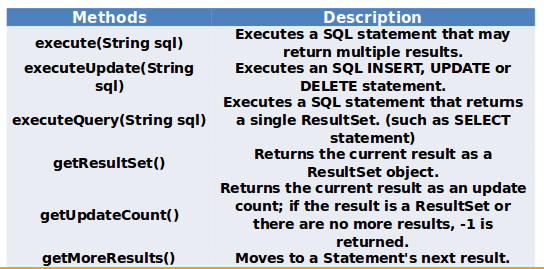
\includegraphics[scale=0.5]{JEE-M03-S01-Image9.png}
  \end{center}
\end{frame}

\begin{frame}[fragile]{Introduction to JDBC}
\begin{block}{}
PreparedStatement Interface
\end{block}
\begin{itemize}
\item Extends the Statement interface
\item Call prepareStatement() method of the Connection interface to create PreparedStatement Object
\item Holds pre-compiled SQL statements
\item Used to execute the SQL statement multiple times
\item Enables us to retrieve, edit, or delete multiple records at a time.
\end{itemize}
\end{frame}

\begin{frame}[fragile]{Introduction to JDBC}
\begin{block}{}
PreparedStatement Interface
\end{block}
\begin{center}
    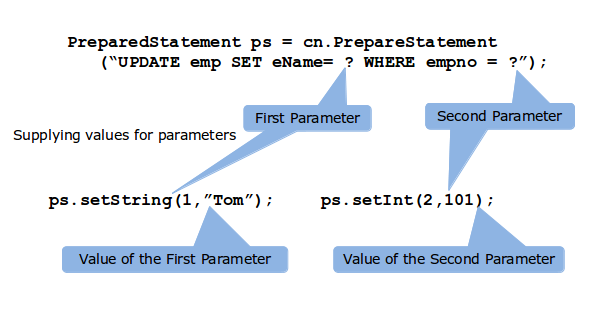
\includegraphics[scale=0.5]{JEE-M03-S01-Image10.png}
  \end{center}
\end{frame}

\begin{frame}[fragile]{Introduction to JDBC}
\begin{block}{}
PreparedStatement Interface
\end{block}
\begin{center}
    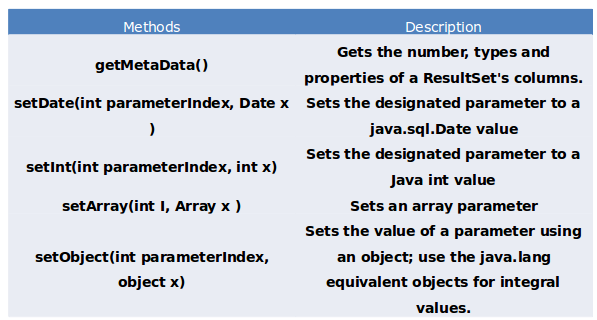
\includegraphics[scale=0.5]{JEE-M03-S01-Image11.png}
  \end{center}
\end{frame}

\begin{frame}[fragile]{Introduction to JDBC}
\begin{block}{}
PreparedStatement Example
\end{block}
\begin{lstlisting}[numbers=none]
Statement stmt = con.createStatement();
String query="UPDATE emp SET eName =? WHERE empno =? ";
PreparedStatement ps=con.prepareStatement(query);
//Here 1 and 2 are the sequential number of values to be set.
ps.setString(1, "Tom");
ps.setInt(2,3);
ps.executeUpdate();
ResultSet rs = stmt.executeQuery("SELECT * FROM emp");
\end{lstlisting}
\end{frame}

\begin{frame}[fragile]{Introduction to JDBC}
\begin{block}{}
CallableStatement Interface
\end{block}
\begin{itemize}
\item Extends the PreparedStatement interface
\item Have a call to a stored procedure 
\item May take IN parameters, OUT Parameters, INOUT parameters.
\item Calling a stored procedure
\end{itemize}
\end{frame}

\begin{frame}[fragile]{Introduction to JDBC}
\begin{itemize}
\item with no parameters
\begin{lstlisting}[numbers=none]
{call procedure_name}
\end{lstlisting}
\item Have a call to a stored procedure 
\begin{lstlisting}[numbers=none]
{ call  procedure_name [(?, ?, ?)]}
\end{lstlisting}
\item May take IN parameters, OUT Parameters, INOUT parameters.
\begin{lstlisting}[numbers=none]
{? = call procedure_name [(?, ?, ?, )]}
\end{lstlisting}
\end{itemize}
\end{frame}

\begin{frame}[fragile]{Introduction to JDBC}
\begin{block}{}
CallableStatement Interface
\end{block}
\begin{itemize}
\item To create a CallableStatement object.
\begin{lstlisting}[numbers=none]
CallableStatement cstmt=cn.prepareCall(“{call procedure_name}”);
\end{lstlisting}
\item Passing IN parameters is done using setXXX() methods
\item Each OUT parameter must be registered in a log file using registerOutParameter() method
\item getXXX() functions OUT parameters are read into application
\end{itemize}
\end{frame}

\begin{frame}[fragile]{Introduction to JDBC}
\begin{block}{}
CallableStatement Interface
\end{block}
\begin{lstlisting}[numbers=none]
CallableStatement ct=cn.prepareCall(“{call getTestData(?,?.?)}”);
ct.registerOutParameter(1,java.sql.Types.TINYINT); // OUT
ct.setFloat(2,1.34);// IN
ct.registerOutParameter(3,java.sql.Types.VARCHAR); // INOUT 
ct.setString(3, “Imran”); // INOUT
ct.executeQuery();
byte x=ct.getBytes(1); // Getting IN
String s=ct.getString(3); // Getting INOUT
\end{lstlisting}
\end{frame}

\begin{frame}[fragile]{Introduction to JDBC}
\begin{block}{}
JDBC Exception Handling
\end{block}
\begin{block}{}
Common exception classes used in the JDBC API:
\end{block}
\begin{itemize}
\item java.sql.SQLException
\begin{itemize}
\item Database access error or other errors
\end{itemize}
\item java.sql.BatchUpdateException
\begin{itemize}
\item Subclass of SQLException 
\item An error occurs during a batch update operation
\end{itemize}
\end{itemize}
\end{frame}

\begin{frame}[fragile]{Introduction to JDBC}
\begin{itemize}
\item java.sql.DataTruncation
\begin{itemize}
\item A data values is unexpectedly truncated for some reasons 
\end{itemize}
\item java.sql.SQLWarning
\begin{itemize}
\item database access warnings  may be retrieved from Connection, Statement and ResultSet objects 
\end{itemize}
\end{itemize}
\end{frame}

\begin{frame}[fragile]{Introduction to JDBC}
\begin{block}{}
Batch Update Facility
\end{block}
\begin{itemize}
\item What is a batch update? 
\begin{itemize}
\item A set of multiple update statements, submitted to the database as a unit.
\end{itemize}
\item Why?
\begin{itemize}
\item It is more efficient to send multiple update.JDBC 2.0 API provides this batch update facility. 
\end{itemize}
\end{itemize}
\end{frame}

\begin{frame}[fragile]{Introduction to JDBC}
\begin{itemize}
\item How?
\begin{description}
\item [addBatch()] of Statement, to add a update statement to Batch.
\item [executeBatch()] of Statement, submits a batch of commands to the database for execution.
\end{description}
\end{itemize}
\end{frame}

\begin{frame}[fragile]{Introduction to JDBC}
\begin{block}{}
Sample Batch Operation
\end{block}
\begin{lstlisting}[numbers=none]
Statement stmt = con.createStatement();
stmt.addBatch("INSERT INTO COFFEES VALUES('Amaretto', 49, 9.99, 0, 0)");
stmt.addBatch("INSERT INTO COFFEES VALUES('Hazelnut', 49, 9.99, 0, 0)");
stmt.addBatch("INSERT INTO COFFEES VALUES('Amaretto_decaf', 49, 10.99, 0, 0)");
stmt.addBatch("INSERT INTO COFFEES VALUES('Hazelnut_decaf', 49, 10.99, 0, 0)");
int [] updateCounts = stmt.executeBatch();
\end{lstlisting}
\end{frame}
\begin{frame}[fragile]{Introduction to JDBC}
\begin{block}{}
Meta data
\end{block}
\begin{itemize}
\item Data about a data is called metadata.
\item Provides information about the Database/ResultSet.
\end{itemize}
\end{frame}

\begin{frame}[fragile]{Introduction to JDBC}
\begin{itemize}
\item Two Interfaces provide following information:
\begin{description}
\item [DatabasesMetaData] Comprehensive information about the database as a whole.
\item [ResultSetMetaData] Information about the types and properties of the columns in a ResultSet object.
\end{description}
\end{itemize}
\end{frame}


\begin{frame}[fragile]{Introduction to JDBC}
\begin{block}{}
DatabaseMetaData
\end{block}
\begin{block}{}
DatabaseMetaData dbmd= con.getMetaData(); 
\end{block}
Method's Description:
\begin{description}
\item [getDatabaseProductName()] Returns the name of the database product.
\end{description}
\end{frame}
\begin{frame}[fragile]{Introduction to JDBC}
\begin{description}
\item [getDatabaseProductVersion()] Returns the version of the database product.
\item [getUserName()] Returns our user name as known tothe database.
\item [getDriverName()] Returns the name of the JDBC driver.
\end{description}
\end{frame}


\begin{frame}[fragile]{Introduction to JDBC}
\begin{description}
\item [getDriverVersion()] Returns the version of the JDBC driver.
\item [getImportedKeys]\textbf{(String catalog, String schema, String table)} Gets a description of the primary key columns that are referenced by a table's foreign key columns (the primary keys imported by a table).
\end{description}
\end{frame}

\begin{frame}[fragile]{Introduction to JDBC}
\begin{block}{}
ResultSetMetaData
\end{block}
\begin{block}{}
ResultSetMetaData rsmd= rs.getMetaData(); 
\end{block}
Method's Description:
\begin{description}
\item [getColumnCount()] Returns the number ofc olumns in this ResultSet.
\end{description}
\end{frame}

\begin{frame}[fragile]{Introduction to JDBC}
\begin{description}
\item [getColumnName(int columnName)] Gets a column's name.
\item [getCoulmnType(int columnName)] Retrieves a column's SQL type.
\item [getTableName(int columnName)] Gets a column's table name.
\item [isCurrency(int columnName)] Indicates whether the column is a cash value.
\end{description}
\end{frame}


\begin{frame}[fragile]{Introduction to JDBC}
\begin{block}{}
Scrollable ResultSets
\end{block}
\begin{itemize}
\item ResultSets have been used in a sequential manner using ResultSet.next()

\end{itemize}

\end{frame}
\begin{frame}[fragile]{Introduction to JDBC}
\begin{itemize}
\item A new method in JDBC allowed to create scrollable and /or update the ResultSets.
\begin{lstlisting}[numbers=none]
createStatement(int resultSetType,int resultSetConcurrency)
\end{lstlisting}
\end{itemize}
\begin{center}
    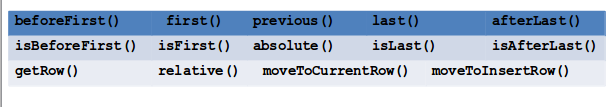
\includegraphics[scale=0.5]{JEE-M03-S01-Image12.png}
  \end{center}
\end{frame}


\begin{frame}[fragile]{Introduction to JDBC}
\begin{block}{}
Scrollable ResultSets
\end{block}
\begin{block}{}
ResultSet Types
\end{block}
\begin{itemize}
\item TYPE\_FORWARD\_ONLY
\begin{itemize}
\item This is the default type which allows only forward movement and columns can be generally read only once.
\end{itemize}
\item TYPE\_SCROLL\_INSENSITIVE
\begin{itemize}
\item Cursor is allowed to move backwards, forwards, and at random
\item Changes are invisible which indicates that the ResultSet is  insensitive.
\end{itemize}
\end{itemize}
\end{frame}

\begin{frame}[fragile]{Introduction to JDBC}
\begin{itemize}
\item TYPE\_SCROLL\_INSENSITIVE
\begin{itemize}
\item Move backwards, forwards, and at random 
\item Allows a dynamic view of data and changes are visible which also means, the ResultSet is sensitive
\end{itemize}
\end{itemize}
\end{frame}

\begin{frame}[fragile]{Introduction to JDBC}
\begin{center}
    
\includegraphics[scale=0.5]{QA.png}
  \end{center}
\end{frame}
\end{document}
